\documentclass[12pt]{article}
\usepackage[utf8]{inputenc}
\usepackage{upquote}
\usepackage[margin=20mm]{geometry} 
\usepackage{amsmath,amsthm,amssymb}
\usepackage{graphicx}
\usepackage{listings}
\newenvironment{statement}[2][Statement]{\begin{trivlist}
\item[\hskip \labelsep {\bfseries #1}\hskip \labelsep {\bfseries #2.}]}{\end{trivlist}}
\usepackage{xcolor}

\usepackage{subfigure}


% Listings package for code rendering (No external dependencies)
\usepackage{listings}  
\usepackage{xcolor}   % Color support
\usepackage{tcolorbox} % Box for better appearance

% Define custom colors for code highlighting
\definecolor{codegreen}{rgb}{0,0.6,0}
\definecolor{codegray}{rgb}{0.5,0.5,0.5}
\definecolor{codepurple}{rgb}{0.58,0,0.82}
\definecolor{backcolour}{rgb}{0.95,0.95,0.92}


\lstset{frame=tb,
    language=Python,
    backgroundcolor=\color{backcolour},   
    commentstyle=\color{codegreen},
    keywordstyle=\color{magenta},
    numberstyle=\tiny\color{codegray},
    stringstyle=\color{codepurple},
    basicstyle=\ttfamily\footnotesize,
    breakatwhitespace=false,         
    breaklines=true,                 
    keepspaces=true,                 
    numbers=left,       
    numbersep=5pt,                  
    showspaces=false,                
    showstringspaces=false,
    showtabs=false,                  
    tabsize=2,
}





\title{Assignment 6}


\author{Author \\
 Wanjing Hu / fng685@alumni.ku.dk  \\
 Shuangcheng Jia / bkg713@alumni.ku.dk/   \\
 Zhigao Yan / sxd343@alumni.ku.dk  \\
} 

\begin{document}
\maketitle

\section{Transformations on images - Translation}
%zhigao


\section{Feature detection and image transforms}
%wanjing
\subsection{}

\textbf{Step1 Preprocess}
We apply Gaussian Blur to reduce noise and smooth out variations. We choose a kernel sized (5,5).
\begin{lstlisting}
image = io.imread(image_path, as_gray=True)
blurred_image = cv2.GaussianBlur(image, (5, 5), 0)  # Kernel size (5,5)
\end{lstlisting}


\textbf{Step2 Corner Detection}
We use Harris Corner Detector to identify key points in the image where intensity changes sharply. The method is set to k to use the Harris response formula, and sigma=1 for standard deviation for Gaussian smoothing. The min distance is set 10 to ensure the detected corners are at least 10 pixels apart. The threshold rel is set to 0.01 to filter weak corner responses.
\begin{lstlisting}
corners_response = corner_harris(blurred_image, method='k', k=0.04, sigma=1)
corners = corner_peaks(corners_response, min_distance=10, threshold_rel=0.01)
\end{lstlisting}

\textbf{Step3 Corner Selection}
The detected points are converted to (x,y) format for processing, and we apply a sorting heuristic  to identify the four primary corners of the label: top-left, top-right, bottom-left, and bottom-right.
\begin{lstlisting}
# Convert (row, col) to (x, y)
corners = np.fliplr(corners)   
# Sort by x, then y
sorted_corners = sorted(corners, key=lambda x: (x[0], x[1])) 
top_left, top_right = sorted_corners[0], sorted_corners[-1]
bottom_left, bottom_right = sorted_corners[1], sorted_corners[-2]
\end{lstlisting}

\textbf{Step4 Estimating Rotation Angle}
The required rotation angle is computed using the atan2 function based on the x-y difference between the top-left and top-right corners. This gives the required rotation angle in degrees, valued -57.28.

\begin{lstlisting}
delta_x = top_right[0] - top_left[0]
delta_y = top_right[1] - top_left[1]
angle = np.arctan2(delta_y, delta_x) * (180.0 / np.pi)  # Convert to degrees
\end{lstlisting}

\textbf{Step5 Image Rotation and Visualization}
Here we plot the detected corners overlayed on the original image. And we display the final rotated image.

The parameter resize=True ensures the entire image remains within frame after rotation. 

Our final result is issued in Figure~\ref{rot}.
\begin{lstlisting}
rotated_image = transform.rotate(image, -angle, resize=True)

fig, ax = plt.subplots(1, 2, figsize=(12, 6))
ax[0].imshow(image, cmap="gray")
ax[0].scatter(corners[:, 0], corners[:, 1], color="red", s=20, label="Corners")
ax[0].set_title("Detected Corners")
ax[0].legend()

ax[1].imshow(rotated_image, cmap="gray")
ax[1].set_title(f"Rotated Image by {-angle:.2f} Degrees")

plt.show()
\end{lstlisting}

% describe the essential steps in your solution including relevant code snippets.

% specify all relevant parameters in the report

% detected label corner points overlayed on top of the image 

% the resulting rotated image and state your estimated rotation angle.

\begin{figure}[h]
    \centering
    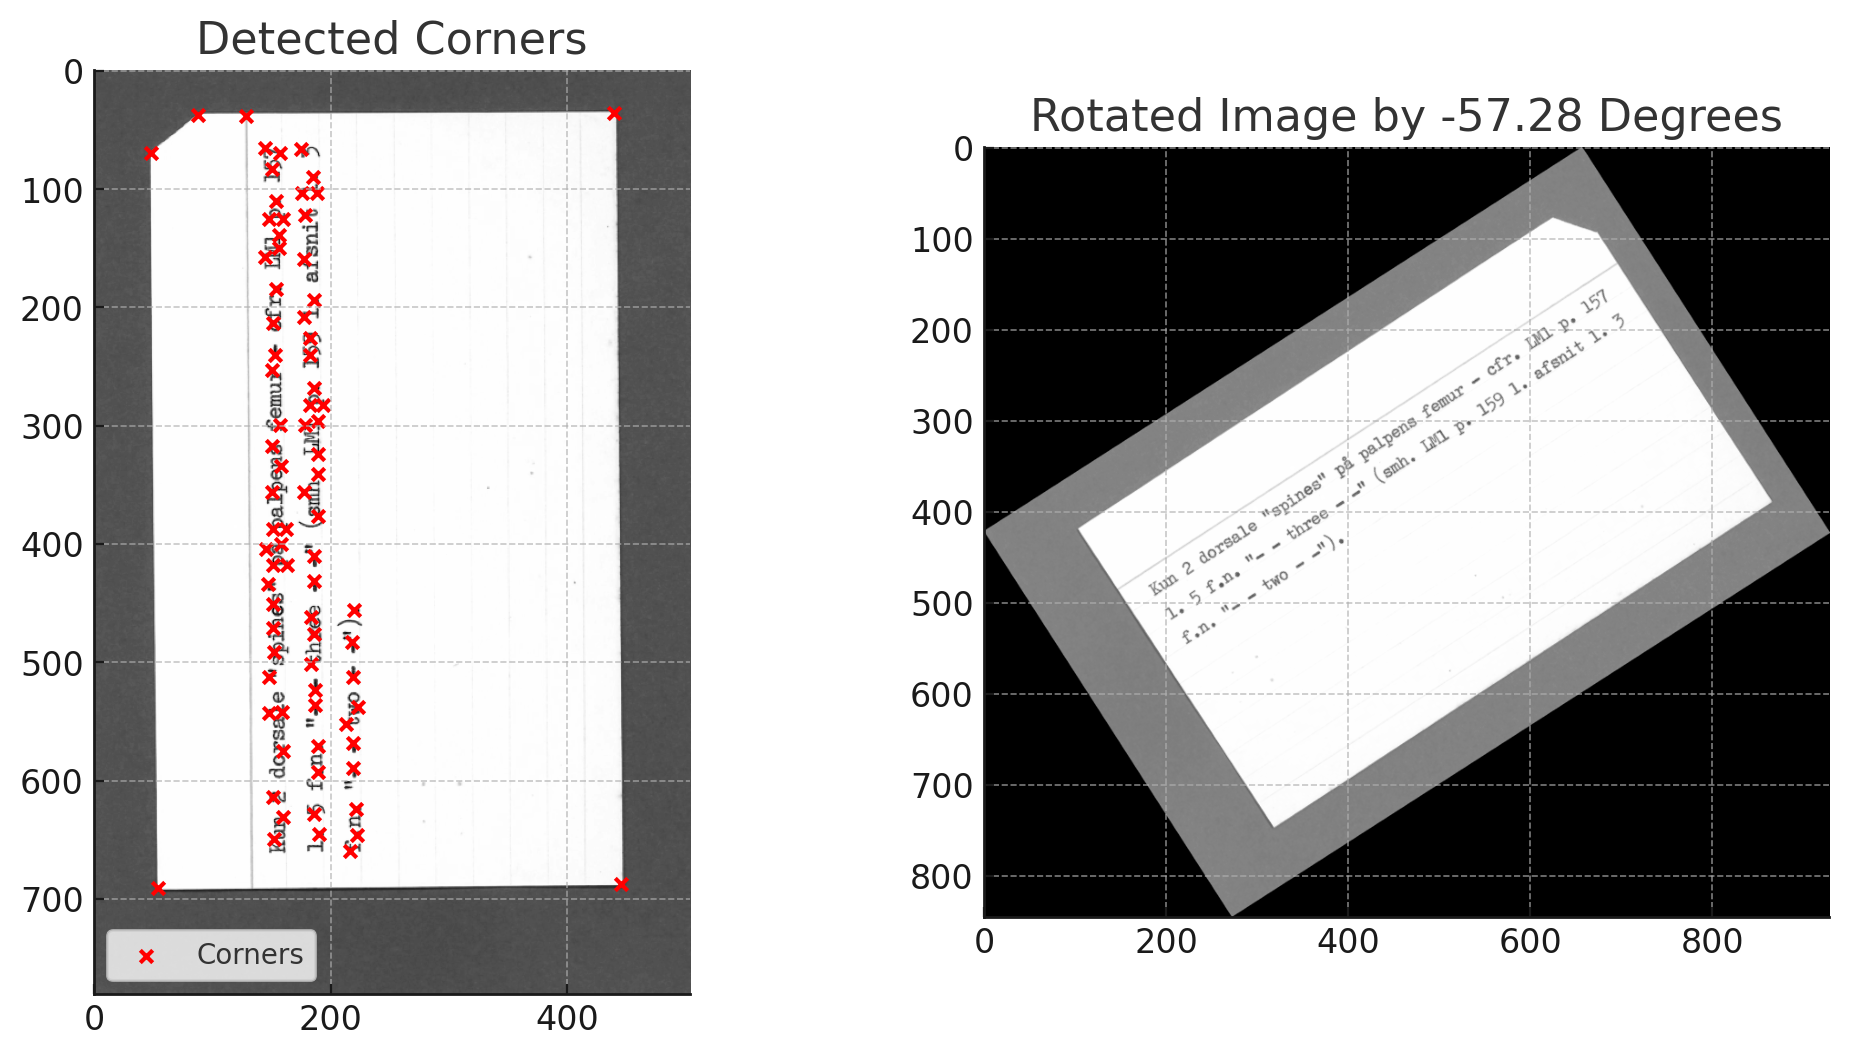
\includegraphics[width=0.8\textwidth]{pics/a6-2.1.png} 
    \caption{Estimated Rotation Angle: -57.28 degrees}
    \label{rot}
\end{figure}


\section{Features, filter banks and texture}
%shuangcheng

\end{document}
